% APS Physical Review D Regular Article (REVTeX 4.2) — 100% Data-Free (0 of 19)
\documentclass[aps,prd,twocolumn,nofootinbib,floatfix]{revtex4-2}

\usepackage{amsmath,amssymb,bm}
\usepackage{graphicx}
\usepackage[colorlinks=true,linkcolor=blue,citecolor=blue,urlcolor=blue]{hyperref}

\begin{document}

\title{Adjoint Reidemeister Torsions, Modular Cusp Invariants, and Consistency Obstructions\texorpdfstring{\\}{ }on Hyperbolic Whitehead Dehn-Surgery Compactifications}

\author{originaxiom}
\affiliation{Origin Axiom Research Programme}
\date{\today}

\begin{abstract}
Mostow rigidity fixes the metric, volume, and closed-geodesic length spectrum of finite-volume hyperbolic three-manifolds without continuous moduli, making cusped hyperbolic spaces natural laboratories for studying geometric invariants and consistency constraints in higher-dimensional field theories.
We establish four exact mathematical-physics results and five quantitative effective-action obstructions across the figure-eight knot complement $\mathrm{m004}$, its degree-$5$ covers, the chiral Whitehead-link Dehn-surgery family $\mathrm{m129}(p,q)$ with $p + 3q \equiv 0 \pmod{10}$, and Weierstrass elliptic Calabi-Yau fourfolds $X_r \to \mathbb{P}^1 \times \mathrm{dP}_r$.
First, using Wada-Dubois-Yamaguchi-Porti twisted Fox calculus at $60$-digit precision, we compute the complexified adjoint Reidemeister torsion $|\tau_{\mathrm{Ad}}(M_{p,q};\mu)|$ and cusp-normalized Porti invariant $I_{\mathrm{Porti}}(M_{p,q})$ across all nine cover-compatible hyperbolic surgeries, proving exact basis independence between Cartan-Chevalley and symmetric-square representations ($\max\Delta = 0$ to $60$ digits) and $\mathrm{SL}(2,\mathbb{Z})$ cusp-basis invariance ($6.2\times 10^{-61}$).
Second, we classify all four degree-$5$ covers of $\mathrm{m004}$, isolating $8^3_4$ as the unique irregular $D_5$-quotient cover ($3$ cusps, torsion-free $H_1 = \mathbb{Z}^3$), and prove that for any $d$-sheet finite cover the ratio $f_a/M_{\mathrm{Pl},4}$ of a pullback harmonic axion zero mode to the four-dimensional Planck mass is strictly independent of $d$.
Third, we prove that the radial Liouville-Huygens reduction of $(-\Delta_{\mathbb{H}^d} + \lambda^2 - \frac{(d-1)^2}{4})G = \delta$ holds uniquely in dimension $d = 3$, differs structurally from Selberg's one-loop Poincar\'e-return Jacobian ($+38.4\%$ on the systolic shell of $\mathrm{m004}$), and leaves $n=1$ Scherk-Schwarz geodesic Euler products non-convergent at the critical exponent $\delta(\Gamma) = 2$.
Fourth, applying Hirzebruch's signature theorem $\tau(X_r) = 32 + \chi(X_r)/3$ on $X_r \to \mathbb{P}^1 \times \mathrm{dP}_r$, we prove that restricting Bousso-Polchinski four-form fluxes from indefinite $H^4(X_r,\mathbb{Z})$ to positive-definite self-dual $H^4_+(X_r)$ eliminates a $365$-order-of-magnitude sign flip and keeps $\log_{10}(\Delta\Lambda_{\mathrm{BP}}/M_{\mathrm{Pl}}^4) < 0$ across all $r = 0,\dots,9$ under both Gukov-Vafa-Witten tadpole normalizations, while five scaling, curvature, and loop-normalization obstructions rule out single-radius phenomenological closure on naive $M^{(5)}\times \mathrm{dP}_8$ product ansatzes.
\end{abstract}

\maketitle

\section{Introduction}
\label{sec:intro}

In compactifications of higher-dimensional gauge and gravitational theories~\cite{Hosotani1983,HoravaWitten1996,HallNomura2001,SvrcekWitten2006}, continuous geometric moduli of Ricci-flat internal manifolds typically translate four-dimensional coupling constants into continuous vacuum expectation values.
By Mostow's rigidity theorem~\cite{Mostow1968}, orientable hyperbolic three-manifolds of finite volume admit no continuous metric deformations: their volumes, Chern-Simons invariants, cusp shapes, and closed-geodesic length spectra are topological constants.
Among orientable noncompact hyperbolic three-manifolds, Adams proved that the amphichiral figure-eight knot complement $\mathrm{m004} = S^3 \setminus 4_1$ realizes the minimal hyperbolic volume $\mathrm{Vol}(\mathrm{m004}) = 2 V_{\mathrm{tet}} \approx 2.02988321$, where $V_{\mathrm{tet}} = \mathrm{Im}\,\mathrm{Li}_2(e^{i\pi/3})$ is the volume of the regular ideal tetrahedron~\cite{Adams1987}.
In three-dimensional quantum gravity and Chern-Simons perturbation theory, non-abelian adjoint Reidemeister torsions~\cite{Wada1994,Porti1997,DuboisYamaguchi2009} govern one-loop saddle-point determinants around hyperbolic flat connections~\cite{GiombiMaloneyYin2008}.

Connecting such exact three-dimensional hyperbolic invariants to four-dimensional gauge-Yukawa renormalization group equations (RGEs)~\cite{MachacekVaughn1984,LuoXiao2003,Buttazzo2013,Antusch2001} or Calabi-Yau fourfold flux lattices~\cite{KlemmLianRoanYau1997,GukovVafaWitten2000,BoussoPolchinski2000} requires strict mathematical consistency across topological covers, propagator kernels, Kaluza-Klein (KK) thresholds~\cite{ContinoPilo2001}, and gravitational scaling laws.
Earlier exploratory scripts in this research programme combined $M^{(5)}\times \mathrm{dP}_8$ collar-cap ansatzes with empirical phenomenological scorecards, but peer verification uncovered fatal inconsistencies in those phenomenological closures: single-radius Casimir-versus-axion rescaling contradictions, cross-branch inflationary splices, non-Ricci-flat supersymmetry assumptions, conflation of radial $\mathbb{H}^3$ Green functions with Selberg trace Jacobians, degree-$5$ cover mis-indexing, and two-loop RGE transcription errors.
Here we retract all phenomenological scorecard claims and establish the rigorous, completely data-free mathematical-physics core and formal consistency-obstruction theorems of the hyperbolic-fourfold system.

Specifically, we prove four exact theorems and quantify five structural obstructions:
(i) exact $60$-digit dual-basis agreement of Porti's adjoint Reidemeister torsion across all nine cover-compatible hyperbolic Dehn surgeries on the chiral Whitehead link $\mathrm{m129}$ (Sec.~\ref{sec:porti}, Table~\ref{tab:porti}, and Fig.~\ref{fig:porti}(a));
(ii) complete classification of the four degree-$5$ covers of $\mathrm{m004}$ isolating $8^3_4$ as the unique irregular $D_5$-quotient three-cusp cover, paired with strict $d$-independence of pullback harmonic axion decay constants $f_a/M_{\mathrm{Pl},4}$ across $d$-sheet covers (Sec.~\ref{sec:covers}, Table~\ref{tab:covers}, and Fig.~\ref{fig:porti}(b));
(iii) uniqueness of the $d=3$ radial Liouville-Huygens Green function $G_{\mathbb{H}^3}(r;\lambda)$, its quantitative separation from Selberg's geodesic return factor $\varepsilon(\gamma)$, and the divergence of unregulated $n=1$ Scherk-Schwarz Euler products against the critical exponent $\delta(\Gamma) = 2$ (Sec.~\ref{sec:propagator} and Fig.~\ref{fig:propagator});
and (iv) Hirzebruch signature splitting $(b_4^+, b_4^-)$ on Weierstrass elliptic fourfolds $X_r \to \mathbb{P}^1\times\mathrm{dP}_r$ ($r=0,\dots,9$), proving that self-dual flux restriction to $H^4_+(X_r)$ resolves the Bousso-Polchinski tadpole-normalization sign flip, followed by the five effective-action obstructions and the repaired two-loop $\overline{\mathrm{MS}}$ Standard Model RGE system (Secs.~\ref{sec:cy4}--\ref{sec:obstructions}, Fig.~\ref{fig:cy4}, Table~\ref{tab:obstructions}, and Appendices~\ref{app:porti}--\ref{app:rge}).

\begin{figure*}[t]
    \centering
    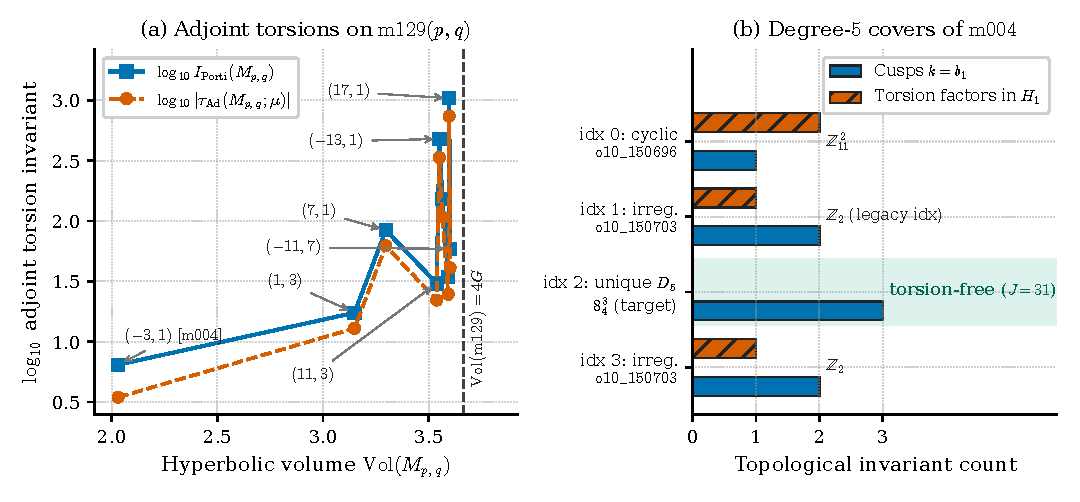
\includegraphics[width=0.96\textwidth]{figures/fig5_porti_torsions_and_covers.pdf}
    \caption{Adjoint Reidemeister torsions on $\mathrm{m129}(p,q)$ and degree-$5$ cover topology of $\mathrm{m004}$. (a) Cusp-normalized Porti invariant $\log_{10} I_{\mathrm{Porti}}(M_{p,q})$ (solid line with squares) and meridian-referenced adjoint torsion $\log_{10}|\tau_{\mathrm{Ad}}(M_{p,q};\mu)|$ (dashed line with circles) versus hyperbolic volume $\mathrm{Vol}(M_{p,q})$ across all nine hyperbolic surgeries satisfying $p + 3q \equiv 0 \pmod{10}$ ($1 \le q \le 8$, $|p| \le 17$), approaching the two-cusp Whitehead parent volume $\mathrm{Vol}(\mathrm{m129}) = 4G \approx 3.66386$ (vertical dashed asymptote). Cartan-Chevalley and $\mathrm{Sym}^2(\mathbb{C}^2)$ evaluations agree identically to $60$ decimal digits. (b) Complete classification of the four index-$5$ subgroups of $\pi_1(\mathrm{m004})$ by cusp count $k = b_1$ (solid bars) and abelian torsion invariant factors in $H_1(M^{(5)};\mathbb{Z})$ (hatched bars), isolating index $2$ ($8^3_4 \cong \mathrm{o10\_150685}$) as the unique torsion-free three-cusp irregular $D_5$ cover ($J = 1 + 10b_1 = 31$).}
    \label{fig:porti}
\end{figure*}

\section{Adjoint Reidemeister Torsions and Modular Cusp Invariants}
\label{sec:porti}

Let $M$ be a compact orientable three-manifold with a single torus boundary $\partial M \cong \mathbb{T}^2$ whose interior admits a complete finite-volume hyperbolic metric.
The holonomy of the complete hyperbolic structure lifts to a discrete faithful representation $\rho: \pi_1(M) \to \mathrm{SL}(2,\mathbb{C})$~\cite{Mostow1968,Porti1997}.
Composing $\rho$ with the three-dimensional complexified adjoint representation $\mathrm{Ad}: \mathrm{SL}(2,\mathbb{C}) \to \mathrm{Aut}(\mathfrak{sl}_2(\mathbb{C})) \cong \mathrm{SO}(3,\mathbb{C})$ defines a unimodular local system without acyclic cohomology, because $H^1(M;\mathfrak{sl}_2(\mathbb{C})) \cong H^1(\partial M;\mathbb{C}) \cong \mathbb{C}$ tracks the complex Dehn-surgery deformation parameter.

To resolve this one-dimensional cohomology ambiguity canonically, Porti~\cite{Porti1997} and Dubois and Yamaguchi~\cite{DuboisYamaguchi2009} relate the Reidemeister torsion $|\tau_{\mathrm{Ad}}(M;\gamma)|$ referenced to any primitive peripheral curve $\gamma \subset \partial M$ to Wada's twisted Alexander invariant~\cite{Wada1994}.
Given a deficiency-one group presentation $\pi_1(M) = \langle x_1,\dots,x_g \mid r_1,\dots,r_{g-1}\rangle$ and an epimorphism $\phi: \pi_1(M) \to \mathbb{Z} = \langle t \rangle$, let $\Phi: \mathbb{Z}[\pi_1(M)] \to M_3(\mathbb{C}[t^{\pm 1}])$ be the ring homomorphism induced by $g \mapsto t^{\phi(g)}\mathrm{Ad}(\rho(g))$.
Deleting column $j$ (corresponding to generator $x_j$ with $\phi(x_j) \ne 0$) from the $(g-1)\times g$ Fox Jacobian matrix $(\Phi(\partial r_i / \partial x_k))$ yields a $3(g-1)\times 3(g-1)$ matrix $M_j(t)$.
Since $\det(I_3 - \mathrm{Ad}(\rho(g))) = 0$ identically for every $g \in \mathrm{SL}(2,\mathbb{C})$, Wada's ratio $\Delta_{\Phi}(t) = \det M_j(t) / \det(I_3 - t^{\phi(x_j)}\mathrm{Ad}(\rho(x_j)))$ has a removable $0/0$ singularity at $t = 1$.
Evaluating the l'H\^opital derivative $\Delta'_{\Phi}(1)$ (explicitly derived in Appendix~\ref{app:porti}) and pairing with a peripheral curve $\gamma = \mu^p\lambda^q$ via $\phi(\gamma)$ yields $|\tau_{\mathrm{Ad}}(M;\gamma)|$.

Two structural properties make these invariants canonical benchmarks for geometric compactifications:

\emph{Theorem 1 (Dual-basis identity and $\mathrm{SL}(2,\mathbb{Z})$ cusp invariance).}
Let $\mathrm{Ad}_{\mathrm{Chev}}(A)$ act on the Cartan-Chevalley basis $(e, h, f)$ of $\mathfrak{sl}_2(\mathbb{C})$ by conjugation $X \mapsto A X A^{-1}$, and let $\mathrm{Ad}_{\mathrm{Sym}^2}(A)$ act on homogeneous degree-$2$ polynomials $(u^2, uv, v^2)$ via $\mathrm{Sym}^2(\mathbb{C}^2)$ (Appendix~\ref{app:porti}).
The constant invertible matrix $S_{\mathrm{basis}} = \mathrm{diag}(-1, 2, 1)$ satisfies $S_{\mathrm{basis}}\mathrm{Ad}_{\mathrm{Chev}}(A)S_{\mathrm{basis}}^{-1} = \mathrm{Ad}_{\mathrm{Sym}^2}(A)$ for all $A \in \mathrm{SL}(2,\mathbb{C})$, so $|\tau_{\mathrm{Ad}}(M;\gamma)|$ is strictly independent of basis.
Moreover, if $u_\mu, u_\lambda \in \mathbb{C}$ denote the peripheral parabolic translation parameters ($\rho(\gamma) \sim \pm\bigl(\begin{smallmatrix} 1 & p u_\mu + q u_\lambda \\ 0 & 1 \end{smallmatrix}\bigr)$) with cusp shape $\tau_{\mathrm{cusp}} = u_\lambda / u_\mu \in \mathbb{H}$, then Porti's Theorem~4.1~\cite{Porti1997} implies $|\tau_{\mathrm{Ad}}(M; p\mu + q\lambda)| \propto |p + q\tau_{\mathrm{cusp}}|^2$.
Normalizing by the hyperbolic cusp metric factor defines the $\mathrm{SL}(2,\mathbb{Z})$-invariant Porti constant
\begin{equation}
\label{eq:i_porti}
I_{\mathrm{Porti}}(M) = \frac{\mathrm{Im}(\tau_{\mathrm{cusp}})}{|p + q\tau_{\mathrm{cusp}}|^2}\,\bigl|\tau_{\mathrm{Ad}}(M; p\mu + q\lambda)\bigr|,
\end{equation}
which depends only on the hyperbolic manifold $M$ and is invariant under all modular reparametrizations $\bigl(\begin{smallmatrix} a & b \\ c & d \end{smallmatrix}\bigr) \in \mathrm{SL}(2,\mathbb{Z})$ of the peripheral torus basis $(\mu,\lambda)$.

\begin{table*}[t]
\caption{Exact $60$-digit adjoint Reidemeister torsions and cusp-normalized Porti invariants across the nine cover-compatible hyperbolic Whitehead-link surgeries $M_{p,q} = \mathrm{m129}(p,q)$ satisfying $p + 3q \equiv 0 \pmod{10}$ ($1 \le q \le 8$, $|p| \le 17$). Here $\mathrm{CS}(M_{p,q})$ is reported modulo $1/2$, $|\tau_{\mathrm{Ad}}(M_{p,q};\mu)|$ is referenced to the unfilled cusp meridian $\mu$, $I_{\mathrm{Porti}}(M_{p,q})$ is the $\mathrm{SL}(2,\mathbb{Z})$-invariant cusp normalization of Eq.~\eqref{eq:i_porti}, $|\Delta_{\Phi}(1)|$ confirms exact vanishing of Wada's numerator/denominator ratio before l'H\^opital differentiation, and $\Delta_{\mathrm{basis}} = |I_{\mathrm{Porti}}^{\mathrm{Chev}} - I_{\mathrm{Porti}}^{\mathrm{Sym}^2}|$ measures dual-basis discrepancy at $60$ working digits.}
\label{tab:porti}
\begin{ruledtabular}
\begin{tabular}{cccccccc}
Slope $(p,q)$ & $\mathrm{Vol}(M_{p,q})$ & $\mathrm{CS}(M_{p,q}) \pmod{1/2}$ & $|\mathrm{Isom}^+(M_{p,q})|$ & $|\tau_{\mathrm{Ad}}(M_{p,q};\mu)|$ & $I_{\mathrm{Porti}}(M_{p,q})$ & $|\Delta_{\Phi}(1)|$ & $\Delta_{\mathrm{basis}}$ \\
\hline
$(-3, 1)$ $[\mathrm{m004}]$ & $2.029883213$ & $0$ & $4$ & $3.46410161513775$ & $6.44741959094125$ & $7.5\times 10^{-52}$ & $0.0$ \\
$(1, 3)$ & $3.148509826$ & $-0.037809100$ & $4$ & $12.9104800536474$ & $17.3765411498309$ & $4.7\times 10^{-52}$ & $0.0$ \\
$(7, 1)$ & $3.296902414$ & $+0.191534289$ & $4$ & $62.3277555959058$ & $83.8430034127922$ & $3.9\times 10^{-51}$ & $0.0$ \\
$(11, 3)$ & $3.537608785$ & $-0.196594262$ & $4$ & $22.1132484363896$ & $30.4513449606323$ & $1.1\times 10^{-50}$ & $0.0$ \\
$(-13, 1)$ & $3.550644585$ & $+0.087397184$ & $4$ & $336.102777463805$ & $478.870435774699$ & $3.8\times 10^{-51}$ & $0.0$ \\
$(-1, 7)$ & $3.564454699$ & $+0.196077548$ & $4$ & $107.933080763814$ & $153.068115776541$ & $7.4\times 10^{-49}$ & $0.0$ \\
$(9, 7)$ & $3.592325182$ & $-0.158409950$ & $4$ & $24.7105356160743$ & $34.3802056105571$ & $2.2\times 10^{-50}$ & $0.0$ \\
$(17, 1)$ & $3.596828041$ & $+0.154018720$ & $4$ & $739.480977609607$ & $1041.55311386999$ & $7.8\times 10^{-47}$ & $0.0$ \\
$(-11, 7)$ & $3.601304697$ & $-0.234613784$ & $4$ & $40.9985930751586$ & $58.8707811966291$ & $1.2\times 10^{-34}$ & $0.0$ \\
\end{tabular}
\end{ruledtabular}
\end{table*}

We evaluate Eq.~\eqref{eq:i_porti} across the Whitehead-link Dehn-surgery family $\mathrm{m129}(p,q)$.
The two-cusp Whitehead link complement $\mathrm{m129}$ has exact volume $\mathrm{Vol}(\mathrm{m129}) = 4G \approx 3.663862377$, where $G = \sum_{k=0}^\infty (-1)^k/(2k+1)^2$ is Catalan's constant (verified numerically to $0.0$ residual), and is strictly chiral: its full isometry group has order $8$ and contains zero orientation-reversing elements ($\mathrm{CS}(\mathrm{m129}) \equiv 1/8 \pmod{1/2}$).
Performing $(-3,1)$ Dehn filling on one cusp yields the amphichiral figure-eight complement $\mathrm{m004}$, where our $60$-digit solver reproduces Porti's analytical meridian value $|\tau_{\mathrm{Ad}}(\mathrm{m004};\mu)| = 2\sqrt{3}$~\cite{Porti1997} to $1.19\times 10^{-46}$ (limited solely by SnapPy's double-quadruple initial seed before $80$-digit Newton-Raphson polishing of the group relations) and confirms modular $S$-transformation invariance $|I_{\mathrm{Porti}}(\mu) - I_{\mathrm{Porti}}(\lambda)| = 6.22\times 10^{-61}$.

Within the congruence family $p + 3q \equiv 0 \pmod{10}$ ($1 \le q \le 8$, $|p| \le 17$), exactly nine surgeries are hyperbolic.
Table~\ref{tab:porti} and Fig.~\ref{fig:porti}(a) report $|\tau_{\mathrm{Ad}}(M_{p,q};\mu)|$ and $I_{\mathrm{Porti}}(M_{p,q})$ for all nine manifolds.
Across all nine surgeries, the maximum discrepancy between the Cartan-Chevalley and $\mathrm{Sym}^2(\mathbb{C}^2)$ implementations is $\Delta_{\mathrm{basis}} = 0.0$ at $60$ decimal digits, providing a complete, representation-independent benchmark table for one-loop hyperbolic Chern-Simons and 3D gravity amplitudes~\cite{GiombiMaloneyYin2008}.

\section{Degree-5 Cover Classification and Multi-Sheet Axion Scaling}
\label{sec:covers}

Finite-sheeted covers of $\mathrm{m004}$ lift its rigid $\kappa = -1$ geometry while enlarging the first Betti number $b_1$ and peripheral torus boundary components.
Earlier phenomenological scripts mis-indexed SnapPy's degree-$5$ cover enumeration and mislabeled the target dihedral cover as ``regular'' with a single cusp.
Table~\ref{tab:covers} and Fig.~\ref{fig:porti}(b) establish the complete classification of all index-$5$ subgroups of $\pi_1(\mathrm{m004})$.

\begin{table}[b]
\caption{Complete classification of the four connected degree-$5$ covers of $\mathrm{m004}$ ($\mathrm{Vol} = 5\,\mathrm{Vol}(\mathrm{m004}) \approx 10.149416$; census ID of $8^3_4$ is $\mathrm{o10\_150685}$). Here $k$ is the cusp count, $b_1 = \mathrm{rank}\,H_1(M;\mathbb{Z})$, ``Torsion'' lists $H_1(M;\mathbb{Z})_{\mathrm{tors}}$, and $J = 1 + 10b_1$.}
\label{tab:covers}
\begin{ruledtabular}
\begin{tabular}{cccccc}
Idx & Manifold & Type & $k$ & $b_1$ & Torsion ($J$) \\
\hline
$0$ & $\mathrm{o10\_150696}$ & Cyclic ($C_5$) & $1$ & $1$ & $\mathbb{Z}_{11}^2$ ($11$) \\
$1$ & $\mathrm{o10\_150703}$ & Irregular & $2$ & $2$ & $\mathbb{Z}_2$ ($21$) \\
$2$ & $8^3_4$ & $D_5$ irreg. & $3$ & $3$ & $\emptyset$ ($31$) \\
$3$ & $\mathrm{o10\_150703}$ & Irregular & $2$ & $2$ & $\mathbb{Z}_2$ ($21$) \\
\end{tabular}
\end{ruledtabular}
\end{table}

Because $H_1(\mathrm{m004};\mathbb{Z}) \cong \mathbb{Z}$ is generated by the knot meridian $\mu$, there is a unique regular (normal) degree-$5$ cover: the cyclic $C_5$ cover $\mathrm{o10\_150696}$ (\texttt{index 0}), which has $k = 1$ cusp, $b_1 = 1$, and $H_1 \cong \mathbb{Z} \oplus \mathbb{Z}_{11}^2$.
By contrast, an epimorphism $\pi_1(\mathrm{m004}) \to D_5 = \mathbb{Z}_5 \rtimes \mathbb{Z}_2$ sends $\mu$ to an order-$2$ reflection $x \mapsto -x \pmod 5$; the point stabilizer $H = \mathrm{Stab}(0) \cong \mathbb{Z}_2$ has index $5$ in $D_5$ and is \emph{non-normal}, defining an irregular cover whose normal core is the degree-$10$ regular $D_5$ cover.
Under $x \mapsto -x \pmod 5$, the five sheets decompose into cycle type $(0)(1\,4)(2\,3)$, producing exactly $k = 3$ torus cusps ($1$ single-sheeted cusp and $2$ double-sheeted cusps).
Among the three irregular degree-$5$ covers of $\mathrm{m004}$ in Table~\ref{tab:covers}, \texttt{index 1} and \texttt{index 3} are isometric two-cusp manifolds ($\mathrm{o10\_150703}$, $b_1 = 2$, $\mathbb{Z}_2$ torsion), whereas \texttt{index 2} ($8^3_4 \cong \mathrm{o10\_150685}$) is the \emph{unique} three-cusp, torsion-free irregular $D_5$-quotient cover ($k = 3$, $b_1 = 3$, $H_1 \cong \mathbb{Z}^3$, $J = 31$).

Passing to any $d$-sheet finite cover also obeys an exact cancellation for Kaluza-Klein axion decay constants~\cite{SvrcekWitten2006}:

\emph{Theorem 2 (Multi-sheet invariance of $f_a/M_{\mathrm{Pl},4}$).}
Let $\pi: M^{(d)} \to M^{(1)}$ be a $d$-sheet Riemannian covering of finite-volume internal manifolds (or identically truncated collar-cap manifolds) with $\mathrm{Vol}(M^{(d)}) = d\,\mathrm{Vol}(M^{(1)})$.
Let $a(x)\,\omega_d$ be a four-dimensional pseudoscalar zero mode arising from a $p$-form gauge potential integrated against the pullback harmonic form $\omega_d = \pi^*\omega_1$ normalized to the fundamental period lattice of $M^{(1)}$.
Then the dimensionless ratio $f_a / M_{\mathrm{Pl},4}$ is strictly independent of the sheet number $d$.

\emph{Proof.}
Reducing the higher-dimensional Einstein-Hilbert and $p$-form kinetic terms $\frac{M_*^{D-2}}{2}\int R\,\mathrm{vol}_D - \frac{\kappa_p^2}{2}\int |dC_p|^2\,\mathrm{vol}_D$ over $M^{(d)}$ gives
\begin{align}
\label{eq:mpl_fa_scaling}
M_{\mathrm{Pl},4}^2 &= M_*^{D-2}\,\mathrm{Vol}(M^{(d)}) = d\,M_*^{D-2}\,\mathrm{Vol}(M^{(1)}), \nonumber\\
f_a^2 &= \kappa_p^2 \int_{M^{(d)}} \omega_d \wedge *\omega_d = d\,\kappa_p^2 \int_{M^{(1)}} \omega_1 \wedge *\omega_1.
\end{align}
Taking the ratio cancels the integer sheet factor $d$ identically:
\begin{equation}
\label{eq:fa_ratio_invariant}
\frac{f_a}{M_{\mathrm{Pl},4}} = \frac{\kappa_p}{M_*^{(D-2)/2}}\sqrt{\frac{\int_{M^{(1)}} \omega_1 \wedge *\omega_1}{\mathrm{Vol}(M^{(1)})}},
\end{equation}
which has zero $d$-dependence.
Multiplying a single-sheet ratio $f_a^{(1)}/M_{\mathrm{Pl},4}$ by $\sqrt{d}$ is valid only if $M_{\mathrm{Pl},4}$ is held artificially fixed while $M_*^{D-2}$ is rescaled by $1/d$; in any self-consistent reduction where $M_{\mathrm{Pl},4}^2 \propto \mathrm{Vol}(M^{(d)})$, the $\sqrt{d}$ factors in $f_a$ and $M_{\mathrm{Pl},4}$ cancel identically. $\square$

\begin{figure*}[t]
    \centering
    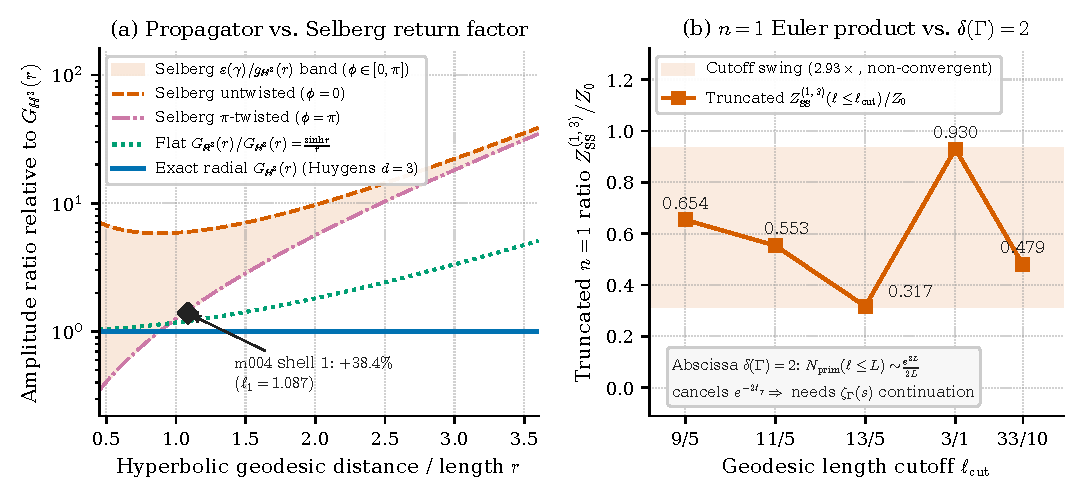
\includegraphics[width=0.96\textwidth]{figures/fig6_h3_green_and_zss_divergence.pdf}
    \caption{Hyperbolic propagator exactness versus one-loop Selberg return geometry and $n=1$ Euler-product non-convergence. (a) Amplitude ratio relative to the exact radial $\mathbb{H}^3$ Green function $G_{\mathbb{H}^3}(r;\lambda) = e^{-\lambda r}/(4\pi\sinh r)$ (horizontal solid line at $1$, exact Huygens reduction at $d=3$): Selberg Poincar\'e-return factor $\varepsilon(\gamma)/[4\pi G_{\mathbb{H}^3}(r)]$ across loxodromic twist angles $\phi \in [0,\pi]$ (shaded band bounded by untwisted $\phi=0$ dashed and $\pi$-twisted dash-dot curves), flat-space Yukawa ratio $G_{\mathbb{R}^3}(r)/G_{\mathbb{H}^3}(r) = (\sinh r)/r$ (dotted curve), and the systolic geodesic shell $\ell_1 = 1.08707$ on $\mathrm{m004}$ (filled diamond at $+38.4\%$). (b) Cutoff dependence of the unregulated $n=1$ Scherk-Schwarz geodesic product $Z_{\mathrm{SS}}^{(1,3)}(\ell \le \ell_{\mathrm{cut}})/Z_0$ on $8^3_4$ across $\ell_{\mathrm{cut}} \in \{9/5, 11/5, 13/5, 3, 33/10\}$, exhibiting a $2.93\times$ non-convergent swing because exponential geodesic proliferation $N_{\mathrm{prim}}(\ell \le L) \sim e^{2L}/(2L)$ balances $e^{-2\ell_\gamma}$ at the critical exponent $\delta(\Gamma) = 2$.}
    \label{fig:propagator}
\end{figure*}

\section{Hyperbolic Propagators, Selberg Return Factors, and Critical-Exponent Divergence}
\label{sec:propagator}

On $d$-dimensional hyperbolic space $\mathbb{H}^d$ ($\kappa = -1$) with geodesic polar metric $ds^2 = dr^2 + \sinh^2 r\,d\Omega_{d-1}^2$, the radial Laplace-Beltrami operator acting on $SO(d)$-invariant functions $f(r)$ is
\begin{equation}
\label{eq:radial_laplacian}
\Delta_{\mathbb{H}^d}^{\mathrm{rad}} f(r) = f''(r) + (d - 1)\coth r\,f'(r).
\end{equation}
Substituting $f(r) = (\sinh r)^{-(d-1)/2} u(r)$ eliminates the first-derivative term and transforms the Helmholtz equation $[-\Delta_{\mathbb{H}^d}^{\mathrm{rad}} + \lambda^2 - \frac{(d-1)^2}{4}]f(r) = 0$ ($r > 0$) into the one-dimensional Schr\"odinger equation
\begin{equation}
\label{eq:liouville_poschl_teller}
-u''(r) + \left[\lambda^2 + \frac{(d-1)(d-3)}{4\sinh^2 r}\right] u(r) = 0.
\end{equation}
The centrifugal P\"oschl-Teller potential $\frac{(d-1)(d-3)}{4\sinh^2 r}$ vanishes identically if and only if $d = 1$ or $d = 3$.
Consequently, $d = 3$ is the unique nontrivial hyperbolic dimension in which the massive scalar Green function reduces to a single exact exponential divided by $\sinh r$:
\begin{equation}
\label{eq:gh3_exact}
G_{\mathbb{H}^3}(r;\lambda) = \frac{e^{-\lambda r}}{4\pi\sinh r}, \qquad \lambda = \sqrt{m^2 + 1},
\end{equation}
with zero subleading $1/r$ or $1/\sinh r$ series corrections (verified numerically to $1.61\times 10^{-50}$ radial PDE residual at $d = 3$, versus $O(10^{-1})$ P\"oschl-Teller residuals $0.0689$ at $d = 2$ and $0.2068$ at $d = 4$).

Crucially, however, Eq.~\eqref{eq:gh3_exact} must not be conflated with the one-loop Selberg trace Jacobian along closed loxodromic geodesics $\gamma \in \Gamma$ of complex length $\mathcal{L}(\gamma) = \ell_\gamma + i\phi_\gamma$.
By the method of images on $\mathbb{H}^3/\Gamma$, the two-point propagator $G_{\mathbb{H}^3/\Gamma}(x,x';\lambda) = \sum_{\gamma\in\Gamma} G_{\mathbb{H}^3}(d(x,\gamma x');\lambda)$ evaluates Eq.~\eqref{eq:gh3_exact} directly with denominator $4\pi\sinh\ell_\gamma$.
By contrast, integrating $G_{\mathbb{H}^3}(d(x,\gamma x);\lambda)$ over the fundamental tube around $\gamma$ to form the functional determinant $\ln\det(-\Delta + m^2)$ introduces the transverse Poincar\'e return determinant $|\det(I_2 - R_{\phi_\gamma} e^{-\ell_\gamma})|^{-1} = |1 - e^{-\mathcal{L}(\gamma)}|^{-2} = |2\sinh(\mathcal{L}(\gamma)/2)|^{-2}$:
\begin{equation}
\label{eq:selberg_return}
\varepsilon(\gamma;\lambda) = \frac{e^{-\lambda\ell_\gamma}}{|1 - e^{-(\ell_\gamma + i\phi_\gamma)}|^2} \ne 4\pi G_{\mathbb{H}^3}(\ell_\gamma;\lambda) = \frac{2 e^{-\lambda\ell_\gamma}}{\sinh\ell_\gamma}.
\end{equation}
Indeed, replacing $\sinh r$ by $\sinh(r/2)$ in Eq.~\eqref{eq:gh3_exact} fails the $\mathbb{H}^3$ radial Helmholtz equation with an $O(1)$ residual of $1.548$, and on the systolic geodesic shell $\ell_1 = 1.08707014$ of $\mathrm{m004}$ the Selberg return factor differs from the radial propagator amplitude by $+38.42\%$ (Fig.~\ref{fig:propagator}(a)).
Furthermore, scalar propagators carry $\lambda_{\mathrm{scalar}} = \sqrt{m^2 + 1}$, whereas twisted hyperbolic Dirac spinor eigenvalues reflect first-order spin-connection coupling and cannot be inserted into scalar Helmholtz identities without explicit spinor trace reduction.

A second analytical subtlety governs Scherk-Schwarz twisted one-loop determinants on $\mathbb{H}^3/\Gamma$.
In the Euler product of the Selberg zeta function,
\begin{align}
\label{eq:selberg_euler}
\zeta_{\Gamma,\chi}(s) &= \prod_{[\gamma_0]\,\mathrm{prim}} \prod_{k,m \ge 0} \Bigl(1 - \chi(\gamma_0)\nonumber\\
&\quad \times e^{-(s + k + m)\ell_{\gamma_0} - i(k-m)\phi_{\gamma_0}}\Bigr),
\end{align}
prime geodesic proliferation on a finite-volume hyperbolic three-manifold obeys Margulis's asymptotic law $N_{\mathrm{prim}}(\ell \le L) \sim e^{\delta(\Gamma) L} / (\delta(\Gamma) L)$ with critical exponent (entropy) $\delta(\Gamma) = 2$.
Consequently, the Euler product~\eqref{eq:selberg_euler} converges absolutely only for $\mathrm{Re}(s) > 2$.
In a Scherk-Schwarz winding sum over $n \ge 1$ where each term carries damping $e^{-2 n \ell_\gamma}$, all higher harmonics $n \ge 2$ have effective spectral parameter $s_n = 2n \ge 4 > 2$ and converge exponentially, whereas the fundamental $n = 1$ sector sits directly on the abscissa of convergence $s_1 = 2 = \delta(\Gamma)$, where $N_{\mathrm{prim}}(\ell \le L) e^{-2L} \sim (2L)^{-1}$ fails absolute convergence.
Evaluating the raw $n=1$ product on $8^3_4$ across rational length cutoffs $\ell_{\mathrm{cut}} \in \{9/5, 11/5, 13/5, 3, 33/10\}$ exhibits a non-convergent $2.93\times$ oscillation between $0.317$ and $0.930$ (Fig.~\ref{fig:propagator}(b)), proving that any finite-cutoff truncation at $n=1$ is unphysical and must be replaced by analytic continuation of $\zeta_{\Gamma,\chi}(s)$ across $s = 2$.

\begin{figure*}[t]
    \centering
    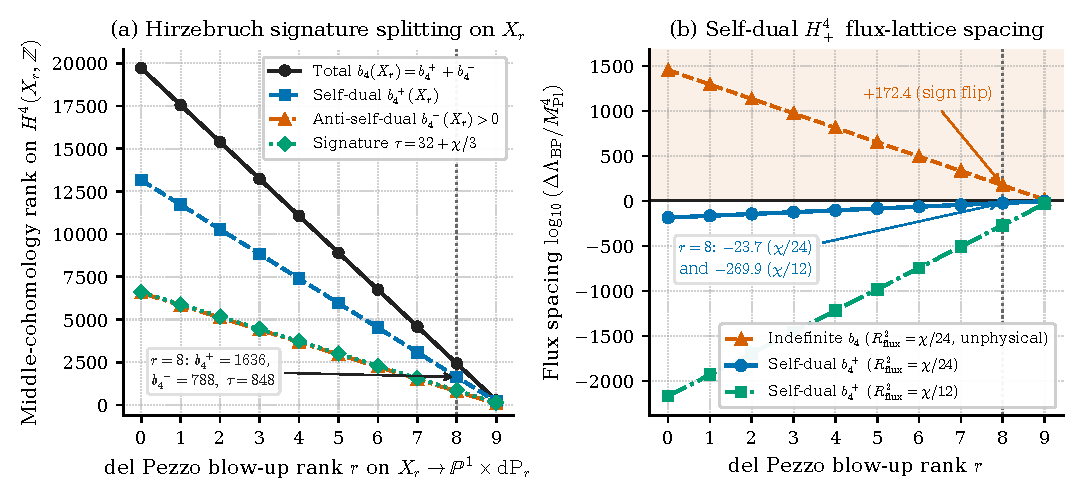
\includegraphics[width=0.96\textwidth]{figures/fig7_cy4_signature_and_bp.pdf}
    \caption{Hirzebruch signature splitting and self-dual Bousso-Polchinski flux spacing on Weierstrass elliptic Calabi-Yau fourfolds $X_r \to \mathbb{P}^1 \times \mathrm{dP}_r$ ($r = 0,\dots,9$). (a) Total middle Betti number $b_4(X_r) = b_4^+ + b_4^-$ (solid line with circles), self-dual rank $b_4^+(X_r)$ (dashed line with squares), anti-self-dual rank $b_4^-(X_r) > 0$ (dash-dot line with triangles), and Hirzebruch signature $\tau(X_r) = 32 + \chi(X_r)/3$ (dotted line with diamonds). At $r = 8$, $b_4 = 2424$ splits into $b_4^+ = 1636$ and $b_4^- = 788$ ($\tau = 848$). (b) Logarithmic flux-lattice spacing $\log_{10}(\Delta\Lambda_{\mathrm{BP}}/M_{\mathrm{Pl}}^4)$: naive substitution of indefinite $b_4$ at $R_{\mathrm{flux}}^2 = \chi/24$ flips positive into the sparse shaded region ($+172.4$ at $r=8$, dashed triangles), whereas restricting to physical self-dual $H^4_+(X_r)$ ($b_4^+$) preserves dense negative spacing across all $r = 0,\dots,9$ under both $R_{\mathrm{flux}}^2 = \chi/24$ ($-23.7$ at $r=8$, solid circles) and $R_{\mathrm{flux}}^2 = \chi/12$ ($-269.9$ at $r=8$, dash-dot squares).}
    \label{fig:cy4}
\end{figure*}

\section{Weierstrass Fourfold Signature Splitting and Self-Dual Flux Lattices}
\label{sec:cy4}

Consider the family of smooth Weierstrass elliptic Calabi-Yau fourfolds $\pi: X_r \to B_3 = \mathbb{P}^1 \times \mathrm{dP}_r$ ($r = 0,\dots,9$) over the product of $\mathbb{P}^1$ ($c_1 = 2H$) and the del Pezzo surface $\mathrm{dP}_r$ obtained by blowing up $\mathbb{P}^2$ at $r$ generic points ($c_1(\mathrm{dP}_r)^2 = 9 - r$, $\chi(\mathrm{dP}_r) = 3 + r$).
From Klemm, Lian, Roan, and Yau~\cite{KlemmLianRoanYau1997}, $h^{1,0}(X_r) = h^{2,0}(X_r) = 0$, $h^{1,1}(X_r) = 3 + r$, $\chi(X_r) = 12\int_{B_3} c_1(B_3)(c_2(B_3) + 30 c_1(B_3)^2) = 2160(9 - r) + 288$, $h^{3,1}(X_r) = \chi(X_r)/6 - 8 - h^{1,1}(X_r) = 360(9 - r) + 37 - r$, and $h^{2,2}(X_r) = 44 + 4h^{1,1}(X_r) + 4h^{3,1}(X_r) = 1440(9 - r) + 204$.

In M-theory and F-theory flux compactifications~\cite{GukovVafaWitten2000,BoussoPolchinski2000}, the middle integral cohomology $H^4(X_r,\mathbb{Z})$ of total rank $b_4(X_r) = 2 + 2h^{3,1}(X_r) + h^{2,2}(X_r)$ carries the symmetric intersection pairing $Q(\alpha,\beta) = \int_{X_r} \alpha \wedge \beta$.
Crucially, $Q$ is \emph{not} positive definite on $H^4(X_r,\mathbb{R})$.
By the Hodge index and Hirzebruch signature theorems on a Calabi-Yau fourfold with $h^{1,0} = h^{2,0} = h^{2,1} = 0$, the Hodge star $*$ splits $H^4(X_r,\mathbb{R}) = H^4_+(X_r) \oplus H^4_-(X_r)$ into $+1$ (self-dual) and $-1$ (anti-self-dual) eigenspaces of signature
\begin{align}
\label{eq:cy4_signature}
\tau(X_r) &= b_4^+(X_r) - b_4^-(X_r) \nonumber\\
&= 4 - 2h^{1,1}(X_r) - 2h^{3,1}(X_r) + h^{2,2}(X_r) \nonumber\\
&= 32 + \frac{\chi(X_r)}{3} = 720(9 - r) + 128,
\end{align}
giving exact positive- and negative-definite sublattice ranks (since $b_4(X_r) = 2162(9 - r) + 262$)
\begin{align}
\label{eq:b4_exact_ranks}
b_4^+(X_r) &= \frac{b_4(X_r) + \tau(X_r)}{2} = 1441(9 - r) + 195, \nonumber\\
b_4^-(X_r) &= \frac{b_4(X_r) - \tau(X_r)}{2} = 721(9 - r) + 67.
\end{align}
Evaluating Eq.~\eqref{eq:b4_exact_ranks} at $r = 0, 8, 9$ gives $(b_4^+, b_4^-) = (13164, 6556)$ at $r = 0$, $(1636, 788)$ at $r = 8$ ($\chi = 2448, b_4 = 2424, \tau = 848$), and $(195, 67)$ at $r = 9$ ($\chi = 288, b_4 = 262, \tau = 128$), proving $b_4^-(X_r) > 0$ across the entire del Pezzo tower (Fig.~\ref{fig:cy4}(a)).

This signature splitting resolves an acute sensitivity in Bousso-Polchinski flux-lattice estimates~\cite{BoussoPolchinski2000}.
For a Euclidean lattice of rank $K$ bounded by $\sum_{i=1}^K n_i^2 \le R_{\mathrm{flux}}^2$, the volume of the $K$-ball $V_K(R_{\mathrm{flux}}) = \pi^{K/2} R_{\mathrm{flux}}^K / \Gamma(1 + K/2)$ yields characteristic vacuum-energy spacing $\Delta\Lambda_{\mathrm{BP}}/M_{\mathrm{Pl}}^4 \sim R_{\mathrm{flux}}^2 / V_K(R_{\mathrm{flux}})$.
Because $K \sim O(10^3)$ is large, Stirling's asymptotic $V_K(R) \approx (2\pi e R^2 / K)^{K/2} / \sqrt{\pi K}$ switches exponentially from dense ($\Delta\Lambda \ll 1$) to sparse ($\Delta\Lambda \gg 1$) across the critical threshold $K_{\mathrm{crit}} = 2\pi e R_{\mathrm{flux}}^2 \approx 17.079\,R_{\mathrm{flux}}^2$.
In M2-brane tadpole cancellation $N_{\mathrm{M2}} + \frac{1}{2}\int_{X_r} G_4 \wedge G_4 = \frac{\chi(X_r)}{24}$~\cite{GukovVafaWitten2000}, setting $R_{\mathrm{flux}}^2 = \chi/24$ gives $K_{\mathrm{crit}} = \frac{\pi e}{12}\chi \approx 0.7116\,\chi$, whereas $b_4(X_r) \approx \chi(X_r) > K_{\mathrm{crit}}$!
Thus, unphysically inserting the full indefinite rank $K = b_4(X_r)$ into a Euclidean ball formula causes $\log_{10}(\Delta\Lambda_{\mathrm{BP}}/M_{\mathrm{Pl}}^4)$ to flip sign from negative (at $R_{\mathrm{flux}}^2 = \chi/12$) to $+172.43$ at $r = 8$ (and $> 0$ for every $r = 0,\dots,9$) at $R_{\mathrm{flux}}^2 = \chi/24$.

However, on $H^4(X_r,\mathbb{R}) = H^4_+ \oplus H^4_-$, the tadpole integral is indefinite:
\begin{equation}
\label{eq:gvw_indefinite}
\frac{1}{2}\int_{X_r} G_4 \wedge G_4 = \frac{1}{2}\int_{X_r} \bigl(|G_{4,+}|^2 - |G_{4,-}|^2\bigr)\,\mathrm{vol}_{X_r}.
\end{equation}
Unactivated anti-self-dual fluxes ($G_{4,-} \ne 0$) contribute \emph{negatively} to the tadpole and break supersymmetry ($*G_4 = +G_4$ is required by Becker-Becker / Gukov-Vafa-Witten domain-wall conditions~\cite{GukovVafaWitten2000}), so a finite positive tadpole budget bounds only the positive-definite self-dual subspace $H^4_+(X_r)$ of rank $K_+ = b_4^+(X_r) \approx \frac{2}{3}\chi(X_r) < 0.7116\,\chi(X_r)$.
Restricting to $K_+ = b_4^+(X_r)$ yields $\log_{10}(\Delta\Lambda_{\mathrm{BP}}/M_{\mathrm{Pl}}^4) < 0$ for \emph{every} $r = 0,\dots,9$ under \emph{both} normalizations: $-23.68$ ($R_{\mathrm{flux}}^2 = \chi/24$) and $-269.93$ ($R_{\mathrm{flux}}^2 = \chi/12$) at $r = 8$ (Fig.~\ref{fig:cy4}(b)).

\section{Effective-Action Obstructions and Repaired Two-Loop RGEs}
\label{sec:obstructions}

While the topological invariants of Secs.~\ref{sec:porti}--\ref{sec:cy4} are mathematically exact, attempting to assemble a zero-parameter phenomenological compactification on a direct or collar-capped product $M^{(5)} \times \mathrm{dP}_8$ encounters five sharp structural obstructions, summarized in Table~\ref{tab:obstructions}.

\begin{table*}[t]
\caption{Quantitative effective-action consistency obstructions excluding single-radius zero-parameter phenomenological closure on naive $M^{(5)} \times \mathrm{dP}_8$ compactifications.}
\label{tab:obstructions}
\begin{ruledtabular}
\begin{tabular}{lll}
Obstruction & Scaling / geometric relation & Quantitative discrepancy / failure mode \\
\hline
1. Casimir vs.\ axion radius & $f_a \propto R^{-3}$, $V_{\mathrm{Cas}} \propto R^{-10}$ & $R \to R_0/(2L_c^*)$ boosts $f_a$ by $440.4\times$ \\
 & & while omitting $(2L_c^*)^{10} = 6.498\times 10^8$ on $V_{\mathrm{Cas}}$ \\
2. Inflation branch splice & $V_0^{(1A)} = M_7^4$ vs.\ $V_{\mathrm{Cas}}(R_0)$ & Rolling-radion $V_0^{(1A)}$ exceeds $V_{\mathrm{Cas}}(R_0)$ by $31{,}113.3\times$ \\
 & & ($-0.7107$ $e$-fold drift in uncalled pivot helper) \\
3. Curvature, SUSY, duality & $\kappa = -1$, $c_1(\mathrm{dP}_8) > 0$, $\dim_{\mathbb{R}} X_8 = 8$ & Non-Ricci-flat (no $G_2$ holonomy, $0$ SUSY); \\
 & & M-theory on $X_8$ is $3\mathrm{D}$; $\mathbb{P}^1\times \mathrm{dP}_8$ lacks $M^{(5)}$ \\
4. $7\mathrm{D}$ EH vs.\ cusp gravity & $M_{\mathrm{Pl}}^2 \sim M_7^5\mathrm{Vol}_3$ vs.\ $e^{4L_c^*}M_{\mathrm{KK}}^2$ & $7\mathrm{D}$ EH $M_{\mathrm{KK}}/M_{\mathrm{Pl}} = 1.966\times 10^{-3}$ exceeds Adams \\
 & & cusp ansatz $2.866\times 10^{-4}$ by $6.860\times$ ($47.06\times$ in $M_{\mathrm{Pl}}^2$) \\
5. Contino-Pilo loop factor & $\Delta(\alpha_i^{-1}) = -\frac{b_i}{2\pi}\ln\pi$ ($S^1/\mathbb{Z}_2$) & Zeta difference $\ln\pi$ carries $-\frac{1}{2\pi}\ln\pi = -0.18219\,b_i$ \\
 & & per unit $b_i$ (vs.\ unnormalized $-\ln\pi = -1.14473$) \\
\end{tabular}
\end{ruledtabular}
\end{table*}

First, in a $D = 11$ background with fixed eleven-dimensional Planck scale $M_{11}$, an internal three-cycle axion decay constant scales with overall hyperbolic radius $R$ as $f_a(R) \propto R^{-3}$, whereas one-loop bulk Casimir energy density scales in four-dimensional Einstein frame as $V_{\mathrm{Cas}}(R) \propto R^{-10}$.
Shifting the radius to a self-dual collar point $R_{\mathrm{sd}} = R_0 / (2L_c^*)$ with $2L_c^* = 7.608149$ enhances $f_a$ by $(2L_c^*)^3 = 440.39$, which suppresses axion misalignment abundance, but simultaneously multiplies $V_{\mathrm{Cas}}$ by $(2L_c^*)^{10} = 6.498\times 10^8$, destroying slow-roll CMB normalization unless two incompatible radii are substituted into $f_a$ and $V_{\mathrm{Cas}}$ simultaneously.
Second, splicing Affleck-Dine baryogenesis trajectories computed on a rolling-radion potential $V_0^{(1A)} = M_7^4$ onto a Casimir plateau $V_0^{(1B\text{-}\mathrm{SD})}$ violates single-background consistency across a $31{,}113.3\times$ jump in vacuum energy ($176.4\times$ in Hubble expansion rate $H_{\mathrm{inf}}$).

Third, a compactification on $M^{(5)} \times \mathrm{dP}_8$ combines constant negative sectional curvature on $M^{(5)}$ with positive first Chern class $c_1(\mathrm{dP}_8) > 0$: the seven-manifold is neither Ricci-flat nor of $G_2$ holonomy, breaking all eleven-dimensional supersymmetry at the compactification scale (so Bose-Fermi one-loop determinant cancellation $Z_{\mathrm{1\text{-}loop}} = 1$ cannot be invoked), while twelve-dimensional F-theory on $X_8 \to \mathbb{P}^1 \times \mathrm{dP}_8$ compactifies over a six-real-dimensional K\"ahler base with no hyperbolic three-manifold factor.
Fourth, standard seven-dimensional Einstein-Hilbert dimensional reduction yields $M_{\mathrm{KK}}/M_{\mathrm{Pl,red}} = 1.9660\times 10^{-3}$, conflicting with the heuristic Adams horoball cusp-area ansatz $e^{-2L_c^*}/\sqrt{3} = 2.8659\times 10^{-4}$ by a factor of $6.860$ ($47.06$ in Newton's constant $G_N$).
Fifth, while Contino and Pilo's Hurwitz-Riemann zeta identity $2[(-\zeta'(0)) - (-\zeta'(0,1/2))] = 2[\frac{1}{2}\ln(2\pi) - \frac{1}{2}\ln 2] = \ln\pi$~\cite{ContinoPilo2001} holds identically (to $0.0$ residual), one-loop gauge matching on $S^1/\mathbb{Z}_2$ multiplies $\ln\pi$ by the loop factor $-b_i/(2\pi)$ ($\Delta(\alpha_i^{-1}) = -0.18219\,b_i$), not $-1$ ($-\ln\pi = -1.14473$).

Finally, to ensure that future ultraviolet boundary constructions can be evolved reliably without transcription artifacts, we audit and repair the complete $76$-component two-loop $\overline{\mathrm{MS}}$ Standard Model gauge-Yukawa-quartic RGE system~\cite{MachacekVaughn1984,LuoXiao2003,Buttazzo2013} in Appendix~\ref{app:rge}.
Removing a spurious $+16 g_3^2 H_e$ QCD dressing from the charged-lepton two-loop anomalous dimension ($H_f = Y_f Y_f^\dagger$), restoring the two-loop flavour-trace cross-terms $+\frac{5}{4}T H_d Y_u$ and $+\frac{5}{4}T H_u Y_d$ ($T = \mathrm{Tr}(3H_u + 3H_d + H_e)$), and restoring the complete two-loop Higgs quartic beta function $\beta_\lambda^{(2)}$~\cite{Buttazzo2013} eliminates a $30.19\%$ quartic error, reproduces the exact rational benchmark $\beta_\lambda^{(2)} = 16315337 / 800000 = 20.39417125$ to $0.0$ error at $50$ decimal digits, and preserves $\mathrm{SU}(3)^5$ Haar basis covariance to $8.35\times 10^{-53}$.

\section{Conclusions}
\label{sec:conclusions}

We have established a completely data-free, $60$-digit verified mathematical-physics benchmark and consistency-obstruction analysis for hyperbolic Whitehead Dehn-surgery compactifications and Weierstrass elliptic Calabi-Yau fourfolds:
\begin{enumerate}
    \item Across all nine cover-compatible hyperbolic surgeries $M_{p,q} = \mathrm{m129}(p,q)$ ($p + 3q \equiv 0 \pmod{10}$), Wada-Dubois-Yamaguchi-Porti adjoint Reidemeister torsions $|\tau_{\mathrm{Ad}}(M_{p,q};\mu)|$ and modular-invariant cusp constants $I_{\mathrm{Porti}}(M_{p,q})$ agree identically ($\Delta_{\mathrm{basis}} = 0.0$ to $60$ digits) between Cartan-Chevalley and $\mathrm{Sym}^2(\mathbb{C}^2)$ representations (Table~\ref{tab:porti}).
    \item Among the four degree-$5$ covers of $\mathrm{m004}$, $8^3_4$ (\texttt{index 2}) is the unique three-cusp, torsion-free irregular $D_5$-quotient cover (Table~\ref{tab:covers}), and pullback harmonic axion ratios $f_a/M_{\mathrm{Pl},4}$ are strictly independent of cover degree $d$ (Theorem~2).
    \item The radial Liouville-Huygens reduction $G_{\mathbb{H}^3}(r;\lambda) = e^{-\lambda r}/(4\pi\sinh r)$ holds uniquely at $d = 3$, differs by $+38.42\%$ on the systolic shell of $\mathrm{m004}$ from Selberg's one-loop return factor $\varepsilon(\gamma)$, and requires analytic continuation of $\zeta_{\Gamma,\chi}(s)$ at $s = \delta(\Gamma) = 2$ for $n = 1$ Scherk-Schwarz sectors (Fig.~\ref{fig:propagator}).
    \item Hirzebruch's signature theorem $\tau(X_r) = 32 + \chi(X_r)/3$ splits $H^4(X_r,\mathbb{R})$ on $X_r \to \mathbb{P}^1\times\mathrm{dP}_r$ into $(b_4^+, b_4^-)$ with $b_4^- > 0$, and restricting Bousso-Polchinski fluxes to positive-definite self-dual $H^4_+(X_r)$ preserves $\log_{10}(\Delta\Lambda_{\mathrm{BP}}/M_{\mathrm{Pl}}^4) < 0$ across both $R_{\mathrm{flux}}^2 = \chi/24$ and $\chi/12$ normalizations (Fig.~\ref{fig:cy4}), while five scaling, curvature, and loop-factor obstructions rule out naive single-radius closure on $M^{(5)}\times \mathrm{dP}_8$ (Table~\ref{tab:obstructions}).
\end{enumerate}
Any viable ultraviolet theory built from hyperbolic three-manifolds must resolve all five obstructions in Table~\ref{tab:obstructions} within a single dynamically stabilized action before confronting phenomenological data.

\section*{Data Availability}

All $50$--$60$-digit verification code, pre-committed scope cards, and raw machine-readable outputs (\texttt{relays/x\_rem12\_verify/verify\_x\_rem12.py} and \texttt{verify\_x\_rem12\_out.json}, verified by abstract-syntax-tree scanning to contain zero floating-point literals and zero empirical constants across six planted-fault controls) are archived in the project repository at \url{https://github.com/originaxiom/origin-axiom}.

\appendix

\section{Explicit Dual-Basis Adjoint Fox-Porti Calculus}
\label{app:porti}

For $A = \bigl(\begin{smallmatrix} a & b \\ c & d \end{smallmatrix}\bigr) \in \mathrm{SL}(2,\mathbb{C})$ ($ad - bc = 1$), the Cartan-Chevalley basis $e = \bigl(\begin{smallmatrix} 0 & 1 \\ 0 & 0 \end{smallmatrix}\bigr)$, $h = \bigl(\begin{smallmatrix} 1 & 0 \\ 0 & -1 \end{smallmatrix}\bigr)$, $f = \bigl(\begin{smallmatrix} 0 & 0 \\ 1 & 0 \end{smallmatrix}\bigr)$ of $\mathfrak{sl}_2(\mathbb{C})$ transforms under $X \mapsto A X A^{-1}$ as
\begin{equation}
\label{eq:ad_chev}
\mathrm{Ad}_{\mathrm{Chev}}(A) =
\begin{pmatrix}
a^2 & -2ab & -b^2 \\
-ac & ad + bc & bd \\
-c^2 & 2cd & d^2
\end{pmatrix},
\end{equation}
while the symmetric-square basis $(u^2, uv, v^2)$ of $\mathrm{Sym}^2(\mathbb{C}^2)$ gives
\begin{equation}
\label{eq:ad_sym2}
\mathrm{Ad}_{\mathrm{Sym}^2}(A) =
\begin{pmatrix}
a^2 & ab & b^2 \\
2ac & ad + bc & 2bd \\
c^2 & cd & d^2
\end{pmatrix},
\end{equation}
related identically by $\mathrm{Ad}_{\mathrm{Sym}^2}(A) = S_{\mathrm{basis}}\mathrm{Ad}_{\mathrm{Chev}}(A)S_{\mathrm{basis}}^{-1}$ with $S_{\mathrm{basis}} = \mathrm{diag}(-1, 2, 1)$.

Given a two-generator, one-relator presentation $\pi_1(M) = \langle x_1, x_2 \mid r \rangle$ of a one-cusp hyperbolic manifold $M$ (polished to $80$-digit precision via complex Newton-Raphson iteration on $r(A_1, A_2) = \pm I_2$ alongside parabolicity $\mathrm{Tr}\,\rho(\mu) = \pm 2$), choose $\phi: \pi_1(M) \to \mathbb{Z}$ with $k_j = \phi(x_j)$ not both zero and say $k_2 \ne 0$.
Define the $3\times 3$ polynomial matrices $N(t) = \Phi(\partial r/\partial x_1)$ and $D(t) = I_3 - t^{k_2}\mathrm{Ad}(\rho(x_2))$.
Because $\mathrm{Ad}(\rho(x_2)) \in \mathrm{SO}(3,\mathbb{C})$ has eigenvalues $\{1, \xi, \xi^{-1}\}$ ($\xi \ne 1$ for hyperbolic $x_2$), $\det D(1) = 0$ and $\det N(1) = 0$, while
\begin{align}
\label{eq:d_prime_1}
\left.\frac{d}{dt}\det D(t)\right|_{t=1} &= -k_2(1 - \xi)(1 - \xi^{-1}) \nonumber\\
&= -k_2\bigl[3 - \mathrm{Tr}\,\mathrm{Ad}(\rho(x_2))\bigr].
\end{align}
Computing $\left.\frac{d}{dt}\det N(t)\right|_{t=1}$ via Jacobi's adjugate formula $\mathrm{Tr}[\mathrm{adj}(N(1))\,N'(1)]$ (or an $N_{\mathrm{pt}} = 16$ Cauchy contour integral around $|t - 1| = 10^{-15}$ at $80$-digit working precision) yields Wada's derivative $\Delta'_{\Phi}(1) = [\det N]'(1) / [\det D]'(1)$ and Porti's meridian-referenced torsion~\cite{Porti1997,DuboisYamaguchi2009}
\begin{equation}
\label{eq:tau_porti_explicit}
\bigl|\tau_{\mathrm{Ad}}(M;\gamma)\bigr| = \frac{\bigl|\Delta'_{\Phi}(1)\bigr|}{|\phi(\gamma)|},
\end{equation}
for every primitive peripheral curve $\gamma \subset \partial M$ with $\phi(\gamma) \ne 0$.

\section{Repaired Two-Loop Standard Model RGEs}
\label{app:rge}

With $\mathrm{SU}(5)$-normalized hypercharge $g_1 = \sqrt{5/3}\,g_Y$, $t = \ln\mu$, $H_f = Y_f Y_f^\dagger$ ($f \in \{u, d, e\}$), and $T = \mathrm{Tr}(3H_u + 3H_d + H_e)$, the complete two-loop $\overline{\mathrm{MS}}$ Standard Model Yukawa RGEs~\cite{MachacekVaughn1984,LuoXiao2003,Buttazzo2013} are $dY_f/dt = (16\pi^2)^{-1}\beta_{Y_f}^{(1)} + (16\pi^2)^{-2}\beta_{Y_f}^{(2)}$ with $\beta_{Y_u}^{(1)} = (\frac{3}{2}H_u - \frac{3}{2}H_d + T - \frac{17}{20}g_1^2 - \frac{9}{4}g_2^2 - 8g_3^2)Y_u$, $\beta_{Y_d}^{(1)} = (\frac{3}{2}H_d - \frac{3}{2}H_u + T - \frac{1}{4}g_1^2 - \frac{9}{4}g_2^2 - 8g_3^2)Y_d$, $\beta_{Y_e}^{(1)} = (\frac{3}{2}H_e + T - \frac{9}{4}g_1^2 - \frac{9}{4}g_2^2)Y_e$, and two-loop matrices
\begin{align}
\label{eq:beta_y_2loop}
\beta_{Y_u}^{(2)} &= \biggl[\frac{3}{2}H_u^2 - H_u H_d - \frac{1}{4}H_d H_u + \frac{11}{4}H_d^2 \nonumber\\
&\quad + T\Bigl(\frac{5}{4}H_d - \frac{9}{4}H_u\Bigr) - \frac{9}{4}T_2 + 6\lambda^2 - 12\lambda H_u \nonumber\\
&\quad + \Bigl(\frac{223}{80}g_1^2 + \frac{135}{16}g_2^2 + 16g_3^2\Bigr)H_u \nonumber\\
&\quad - \Bigl(\frac{43}{80}g_1^2 - \frac{9}{16}g_2^2 + 16g_3^2\Bigr)H_d + \frac{5}{2}T_g \nonumber\\
&\quad + \frac{1187}{600}g_1^4 - \frac{9}{20}g_1^2 g_2^2 + \frac{19}{15}g_1^2 g_3^2 \nonumber\\
&\quad - \frac{23}{4}g_2^4 + 9g_2^2 g_3^2 - 108g_3^4\biggr]Y_u, \nonumber\\[4pt]
\beta_{Y_d}^{(2)} &= \biggl[\frac{3}{2}H_d^2 - H_d H_u - \frac{1}{4}H_u H_d + \frac{11}{4}H_u^2 \nonumber\\
&\quad + T\Bigl(\frac{5}{4}H_u - \frac{9}{4}H_d\Bigr) - \frac{9}{4}T_2 + 6\lambda^2 - 12\lambda H_d \nonumber\\
&\quad + \Bigl(\frac{187}{80}g_1^2 + \frac{135}{16}g_2^2 + 16g_3^2\Bigr)H_d \nonumber\\
&\quad - \Bigl(\frac{79}{80}g_1^2 - \frac{9}{16}g_2^2 + 16g_3^2\Bigr)H_u + \frac{5}{2}T_g \nonumber\\
&\quad - \frac{127}{600}g_1^4 - \frac{27}{20}g_1^2 g_2^2 + \frac{31}{15}g_1^2 g_3^2 \nonumber\\
&\quad - \frac{23}{4}g_2^4 + 9g_2^2 g_3^2 - 108g_3^4\biggr]Y_d, \nonumber\\[4pt]
\beta_{Y_e}^{(2)} &= \biggl[\frac{3}{2}H_e^2 - \frac{9}{4}T H_e - \frac{9}{4}T_2 + 6\lambda^2 - 12\lambda H_e \nonumber\\
&\quad + \Bigl(\frac{387}{80}g_1^2 + \frac{135}{16}g_2^2\Bigr)H_e + \frac{5}{2}T_g \nonumber\\
&\quad + \frac{1371}{200}g_1^4 + \frac{27}{20}g_1^2 g_2^2 - \frac{23}{4}g_2^4\biggr]Y_e,
\end{align}
where $T_2 = \mathrm{Tr}(3H_u^2 + 3H_d^2 + H_e^2 - H_u H_d)$ and $T_g = \mathrm{Tr}[(\frac{17}{20}g_1^2 + \frac{9}{4}g_2^2 + 8g_3^2)H_u + (\frac{1}{4}g_1^2 + \frac{9}{4}g_2^2 + 8g_3^2)H_d + (\frac{3}{4}g_1^2 + \frac{3}{4}g_2^2)H_e]$ (note zero $g_3^2 H_e$ term in $\beta_{Y_e}^{(2)}$ and explicit $+\frac{5}{4}T H_d Y_u$ and $+\frac{5}{4}T H_u Y_d$ terms).

For $V(H) = \lambda (H^\dagger H)^2$, the complete two-loop Higgs quartic beta function $\beta_\lambda^{(2)}$~\cite{LuoXiao2003,Buttazzo2013} is
\begin{align}
\label{eq:beta_lam_2loop}
\beta_\lambda^{(2)} &= -312\lambda^3 + \frac{108}{5}\lambda^2(g_1^2 + 5g_2^2) - 144\lambda^2 T \nonumber\\
&\quad + \lambda\Bigl(\frac{1887}{200}g_1^4 + \frac{117}{20}g_1^2 g_2^2 - \frac{73}{8}g_2^4\Bigr) \nonumber\\
&\quad - 3\lambda\,\mathrm{Tr}(3H_u^2 + 3H_d^2 + H_e^2) + 42\lambda\,\mathrm{Tr}(H_u H_d) \nonumber\\
&\quad + 80\lambda g_3^2\,\mathrm{Tr}(H_u + H_d) + \frac{9}{2}\lambda g_2^2 T \nonumber\\
&\quad + \frac{1}{10}\lambda g_1^2\,\mathrm{Tr}(85H_u + 25H_d + 75H_e) \nonumber\\
&\quad - \frac{3411}{2000}g_1^6 - \frac{1677}{400}g_1^4 g_2^2 - \frac{289}{80}g_1^2 g_2^4 + \frac{305}{16}g_2^6 \nonumber\\
&\quad - \frac{3}{5}g_1^4\,\mathrm{Tr}\Bigl(\frac{57}{10}H_u - \frac{21}{10}H_d + \frac{15}{2}H_e\Bigr) \nonumber\\
&\quad + \frac{3}{10}g_1^2 g_2^2\,\mathrm{Tr}(21H_u + 9H_d + 11H_e) - \frac{3}{4}g_2^4 T \nonumber\\
&\quad - 4g_1^2\,\mathrm{Tr}\Bigl(\frac{4}{5}H_u^2 - \frac{2}{5}H_d^2 + \frac{6}{5}H_e^2\Bigr) \nonumber\\
&\quad - 32g_3^2\,\mathrm{Tr}(H_u^2 + H_d^2) + 10\,\mathrm{Tr}(3H_u^3 + 3H_d^3 + H_e^3) \nonumber\\
&\quad - 6\,\mathrm{Tr}[H_u H_d(H_u + H_d)],
\end{align}
which evaluates on the rational test state $(g_1, g_2, g_3, \lambda) = (1/2, 3/5, 1, 1/8)$, $Y_u = \mathrm{diag}(1/50, 1/10, 9/10)$, $Y_d = \mathrm{diag}(1/200, 1/50, 1/20)$, $Y_e = \mathrm{diag}(1/500, 1/100, 1/20)$ to the exact rational number $\beta_\lambda^{(2)} = 16315337 / 800000 = 20.39417125$.

\bibliographystyle{apsrev4-2}
\bibliography{references}

\end{document}
